\documentclass{article}

\title{Forecasting Seasonal Influenza in the U.S.: A colalborative multi-year, multi-model assessment of forecast performance}

\author{Logan Brooks, Spencer Fox, Sasikiran Kandula, Craig McGowan, Evan Moore, \\Dave Osthus, Evan Ray, Nicholas G Reich, Roni Rosenfeld, Jeffrey Shaman, \\Abhinav Tushar, Teresa Yamana [authorship list to be finalized]}

\usepackage[letterpaper, margin=1in]{geometry} % margin
\usepackage{lineno}% add line numbers
\usepackage{graphicx}
\usepackage[colorlinks=true, allcolors=blue]{hyperref}
\usepackage{parskip}        % for spacing after paragraphs http://ctan.org/pkg/parskip
\usepackage{url}            % simple URL typesetting
\usepackage{booktabs}       % professional-quality tables
\usepackage{amsfonts}       % blackboard math symbols
\usepackage{nicefrac}       % compact symbols for 1/2, etc.
\usepackage{amsmath, amsfonts}
\usepackage{setspace}
\linenumbers % line numbers
\onehalfspacing



% For computer modern sans serif
\usepackage[T1]{fontenc}
\renewcommand*\familydefault{\sfdefault} %% Only if the base font of the document is to be sans serif


\usepackage{Sweave}
\begin{document}
\input{comparison-manuscript-concordance}

\maketitle

\begin{abstract}

TBD.

\end{abstract}
%\tableofcontents


\begin{Schunk}
\begin{Sinput}
> scores <- read_csv("../../scores/scores.csv")
> models <- read_csv("../../model-forecasts/component-models/model-id-map.csv")
> targets <- read_csv("../../scores/target-multivals.csv")
> complete_models <- c(models$`model-id`[models$complete=="true"], "UTAustin-edm")
> compartment_models <- c("CU-EAKFC_SEIRS", "CU-EAKFC_SIRS", "CU-EKF_SEIRS", 
+     "CU-EKF_SIRS", "CU-RHF_SEIRS", "CU-RHF_SIRS", "LANL-DBM")
> ## define column with scores of interest
> SCORE_COL <- quo(`Multi bin score`)
> ## Create data.frame of boundary weeks of scores to keep for each target/season
> all_target_bounds <- read_csv("data/all-target-bounds.csv")
> ## Remove scores that fall outside of evaluation period for a given target/season
> scores_trimmed <- scores %>% 
+     dplyr::left_join(all_target_bounds, by = c("Season", "Target", "Location")) %>%
+     dplyr::filter(`Model Week` >= start_week_seq, `Model Week` <= end_week_seq)
> ## truncate lowest possible scores to -10, define target-type variable
> scores_adj <- scores_trimmed %>%
+     filter(Model %in% complete_models) %>%
+     ## if NA, NaN or <-10, set score to -10
+     mutate(score_adj = dplyr::if_else(is.nan(!!SCORE_COL) | is.na(!!SCORE_COL) , 
+         -10, 
+         !!SCORE_COL),
+         target_type = dplyr::if_else(Target %in% c("Season onset", "Season peak week", "Season peak percentage"),
+             "seasonal", "k-week-ahead")) %>%
+     mutate(
+         score_adj = dplyr::if_else(score_adj < -10 , -10, score_adj),
+         Location = factor(Location, levels=c("US National", paste("HHS Region", 1:10))),
+         model_type = ifelse(Model %in% compartment_models, "compartment_model", "stat_model"),
+         stat_model = ifelse(Model %in% compartment_models, 0, 1)
+         ) 
> scores_by_model <- scores_adj %>%
+     group_by(Model) %>%
+     summarize(
+         avg_logscore = mean(score_adj)
+     ) %>%
+     ungroup() %>%
+     mutate(Model = reorder(Model, avg_logscore))
> scores_by_model_target <- scores_adj %>%
+     group_by(Model, Target) %>%
+     summarize(
+         avg_logscore = mean(score_adj)
+     ) %>%
+     ungroup() %>%
+     mutate(Model = reorder(Model, avg_logscore))
> scores_by_model_season <- scores_adj %>%
+     group_by(Model, Season) %>%
+     summarize(
+         avg_logscore = mean(score_adj)
+     ) %>%
+     ungroup() %>%
+     mutate(Model = reorder(Model, avg_logscore))
> scores_by_model_targettype <- scores_adj %>%
+     group_by(Model, target_type) %>%
+     summarize(
+         avg_logscore = mean(score_adj)
+     ) %>%
+     ungroup() %>%
+     mutate(Model = reorder(Model, avg_logscore))
> scores_by_model_region <- scores_adj %>%
+     group_by(Model, Location) %>%
+     summarize(
+         avg_logscore = mean(score_adj)
+     ) %>%
+     ungroup() %>%
+     mutate(Model = reorder(Model, avg_logscore))
> scores_by_model_season_target <- scores_adj %>%
+     group_by(Model, Season, Target) %>%
+     summarize(
+         avg_logscore = mean(score_adj)
+     ) %>%
+     ungroup() %>%
+     mutate(Model = reorder(Model, avg_logscore))
> scores_by_model_season_target_region <- scores_adj %>%
+     group_by(Model, Season, Target, Location) %>%
+     summarize(
+         avg_logscore = mean(score_adj)
+     ) %>%
+     ungroup() %>%
+     mutate(Model = reorder(Model, avg_logscore))
> scores_by_model_targettype_region <- scores_adj %>%
+     group_by(Model, target_type, Location) %>%
+     summarize(
+         avg_logscore = mean(score_adj)
+     ) %>%
+     ungroup() %>%
+     mutate(Model = reorder(Model, avg_logscore))
> scores_by_model_season_targettype_region <- scores_adj %>%
+     group_by(Model, Season, target_type, Location) %>%
+     summarize(
+         avg_logscore = mean(score_adj)
+     ) %>%
+     ungroup() %>%
+     mutate(Model = reorder(Model, avg_logscore))
> scores_by_region <- scores_adj %>%
+     group_by(Location) %>%
+     summarize(
+         avg_logscore = mean(score_adj)
+     ) %>%
+     ungroup() %>%
+     mutate(Location = reorder(Location, avg_logscore))
> scores_by_season <- scores_adj %>%
+     group_by(Season) %>%
+     summarize(
+         avg_logscore = mean(score_adj)
+     ) %>%
+     ungroup() %>%
+     mutate(Season = reorder(Season, avg_logscore))
> scores_by_region_targettype <- scores_adj %>%
+     group_by(Location, target_type) %>%
+     summarize(
+         avg_logscore = mean(score_adj)
+     ) %>%
+     ungroup() %>%
+     mutate(Location = reorder(Location, avg_logscore))
\end{Sinput}
\end{Schunk}



\section{Introduction}

Over the past 15 years, the number of published research articles on forecasting infectious diseases has tripled (Web of Science). 
This increased interest has been fueled in part by the promise of `big data', that near real-time data streams of large-scale population behavior \cite{Molodecky2017} to microscopic changes in a pathogen \cite{Du2017} could lead to measurable improvements in how disease transmission is measured, forecasted, and prevented \cite{Bansal2016}. 
With the spectre of a global pandemic looming, improving infectious disease forecasting continues to be a central priority of global health preparedness efforts.\cite{Myers2000,WorldHealthOrganization2016,Chretien2015}

Forecasts of infectious disease transmission can inform public health response to outbreaks. 
Accurate forecasts of the timing and spatial spread of outbreaks of infectious diseases can provide valuable information about where public health interventions can be targeted.\cite{Lipsitch2011}
Decisions about hospital staffing, resource allocation, and the timing of public health communication campaigns can be assisted by forecasts. 
Implementation of interventions designed to disrupt disease transmission, such as vector control measures or mandatory infection prevention protocols at hospitals or health clinics, can be targeted based on forecasted incidence.

In part due to the growing recognition of the importance of systematically integrating forecasting into public health outbreak response, large-scale collaborations have been used in forecasting applications to develop common data standards and facilitate comparisons across multiple models.\cite{Biggerstaff2016,Smith2017,Biggerstaff2018,Viboud2017}
%These studies serve as an important counterweight to many forecasting efforts remain one-off academic exercises focused on a single application or a single method.
By enabling a standardized comparison in a single application, these studies greatly improve our understanding of which models perform best in certain settings, of how results can best be disseminated and used by decision-makers, and of what the bottlenecks are in terms of improving forecasts.

The aim of this study is to present a standardized comparison of a range of different forecasting models for influenza in the US, over multiple seasons.
Our work brings together models from five different institutions: Carnegie Mellon, Columbia University, Los Alamos National Laboratory, University of Massachusetts-Amherst, and University of Texas-Austin.
While most groups developed more than one model for consideration, the models developed within a single group through the use of common data sources and/or methodologies often bear similarities to each other.
Having 22 models from five different teams enhances the diversity of the models presented.

While such multi-model comparisons exist in the literature for single-season performance, a unique aspect of this work is its focus on performance of the models over a longer period of time, i.e. seven flu seasons. 
To our knowledge, this is the first documented comparison of multiple models (from different teams), in a ``real-time'' setting, across multiple seasons for any infectious disease application.
Since each season has unique dynamical structure, multi-season comparisons like this have great potential to improve our understanding of how models perform over the longer term and which models may be reliable in the future.

This work relies on the forecasting structure developed by existing public forecasting challenges.
Starting in the 2013/2014 influenza season, the U.S. Centers for Disease Control and Prevention (CDC) has run the "Forecast the Influenza Season Collaborative Challenge" (a.k.a. FluSight) each influenza season, soliciting weekly forecasts for specific influenza season metrics from teams across the world.\cite{Biggerstaff2016,Biggerstaff2018}
These forecasts are displayed together on a website during the season and are evaluated for accuracy after the season is over.\cite{PhiResearchLab} 
This effort has galvanized a community of scientists interested in forecasting, creating an organic testbed for improving both our technical understanding of how different forecast models perform and also how to integrate these models into decision-making.


Building on the structure of the FluSight challenges (and those of other collaborative forecasting efforts\cite{Smith2017,Viboud2017}), a subset of FluSight participants founded a consortium in early 2017 to facilitate direct comparison and fusion of modeling approaches. 
In this paper, we provide a detailed analysis of the performance of 22 different models from five different teams over the course of seven influenza seasons.
Drawing on the different expertise of the five teams allows us to make fine-grained and standardized comparisons of distinct approaches to disease incidence forecasting that use different data sources and statistical models.

In addition to analyzing comparative model performance over seasons, this work identifies key bottlenecks that limit the accuracy and generalizability of current forecasting efforts.
Specifically, we present quantitative analyses of the impact that incomplete or partial case reporting has on forecast accuracy.
Additionally, we assess whether purely statistical models show similar performance to models that consider explicit mechanistic models of disease transmission.


\section{Methods}

\subsection{FluSight Challenge Overview}
 
Detailed methodology and results from previous FluSight challenges have been published\cite{Biggerstaff2016,Biggerstaff2018}, and we summarize the key features of the challenge here.

The FluSight challenge focuses on forecasts of the weighted percentage of doctor's office visits where the patient showed symptoms of an influenza-like illness in a particular region. Weighting is done by state population as the data are aggregated to the regional level.
This is a standard measure of seasonal flu activity, for which public data is available for the US back to the 1997/1998 influenza season (Figure \ref{fig:intro-schematic}A). 
During each influenza season, these data are updated each week by the CDC. When the most recent data are released, the prior weeks' reported wILI data may also be revised. 
The unrevised data, available at a particular moment in time, is available via the DELPHI real-time epidemiological data API beginning in the 2013/2014 season.\cite{DELPHI} 
This API enables researchers to ``turn back the clock'' to a particular moment in time and use the data available at that time. This tool facilitates more accurate assessment of how models would have performed in real-time. 

\begin{figure}[htbp]
\begin{center}
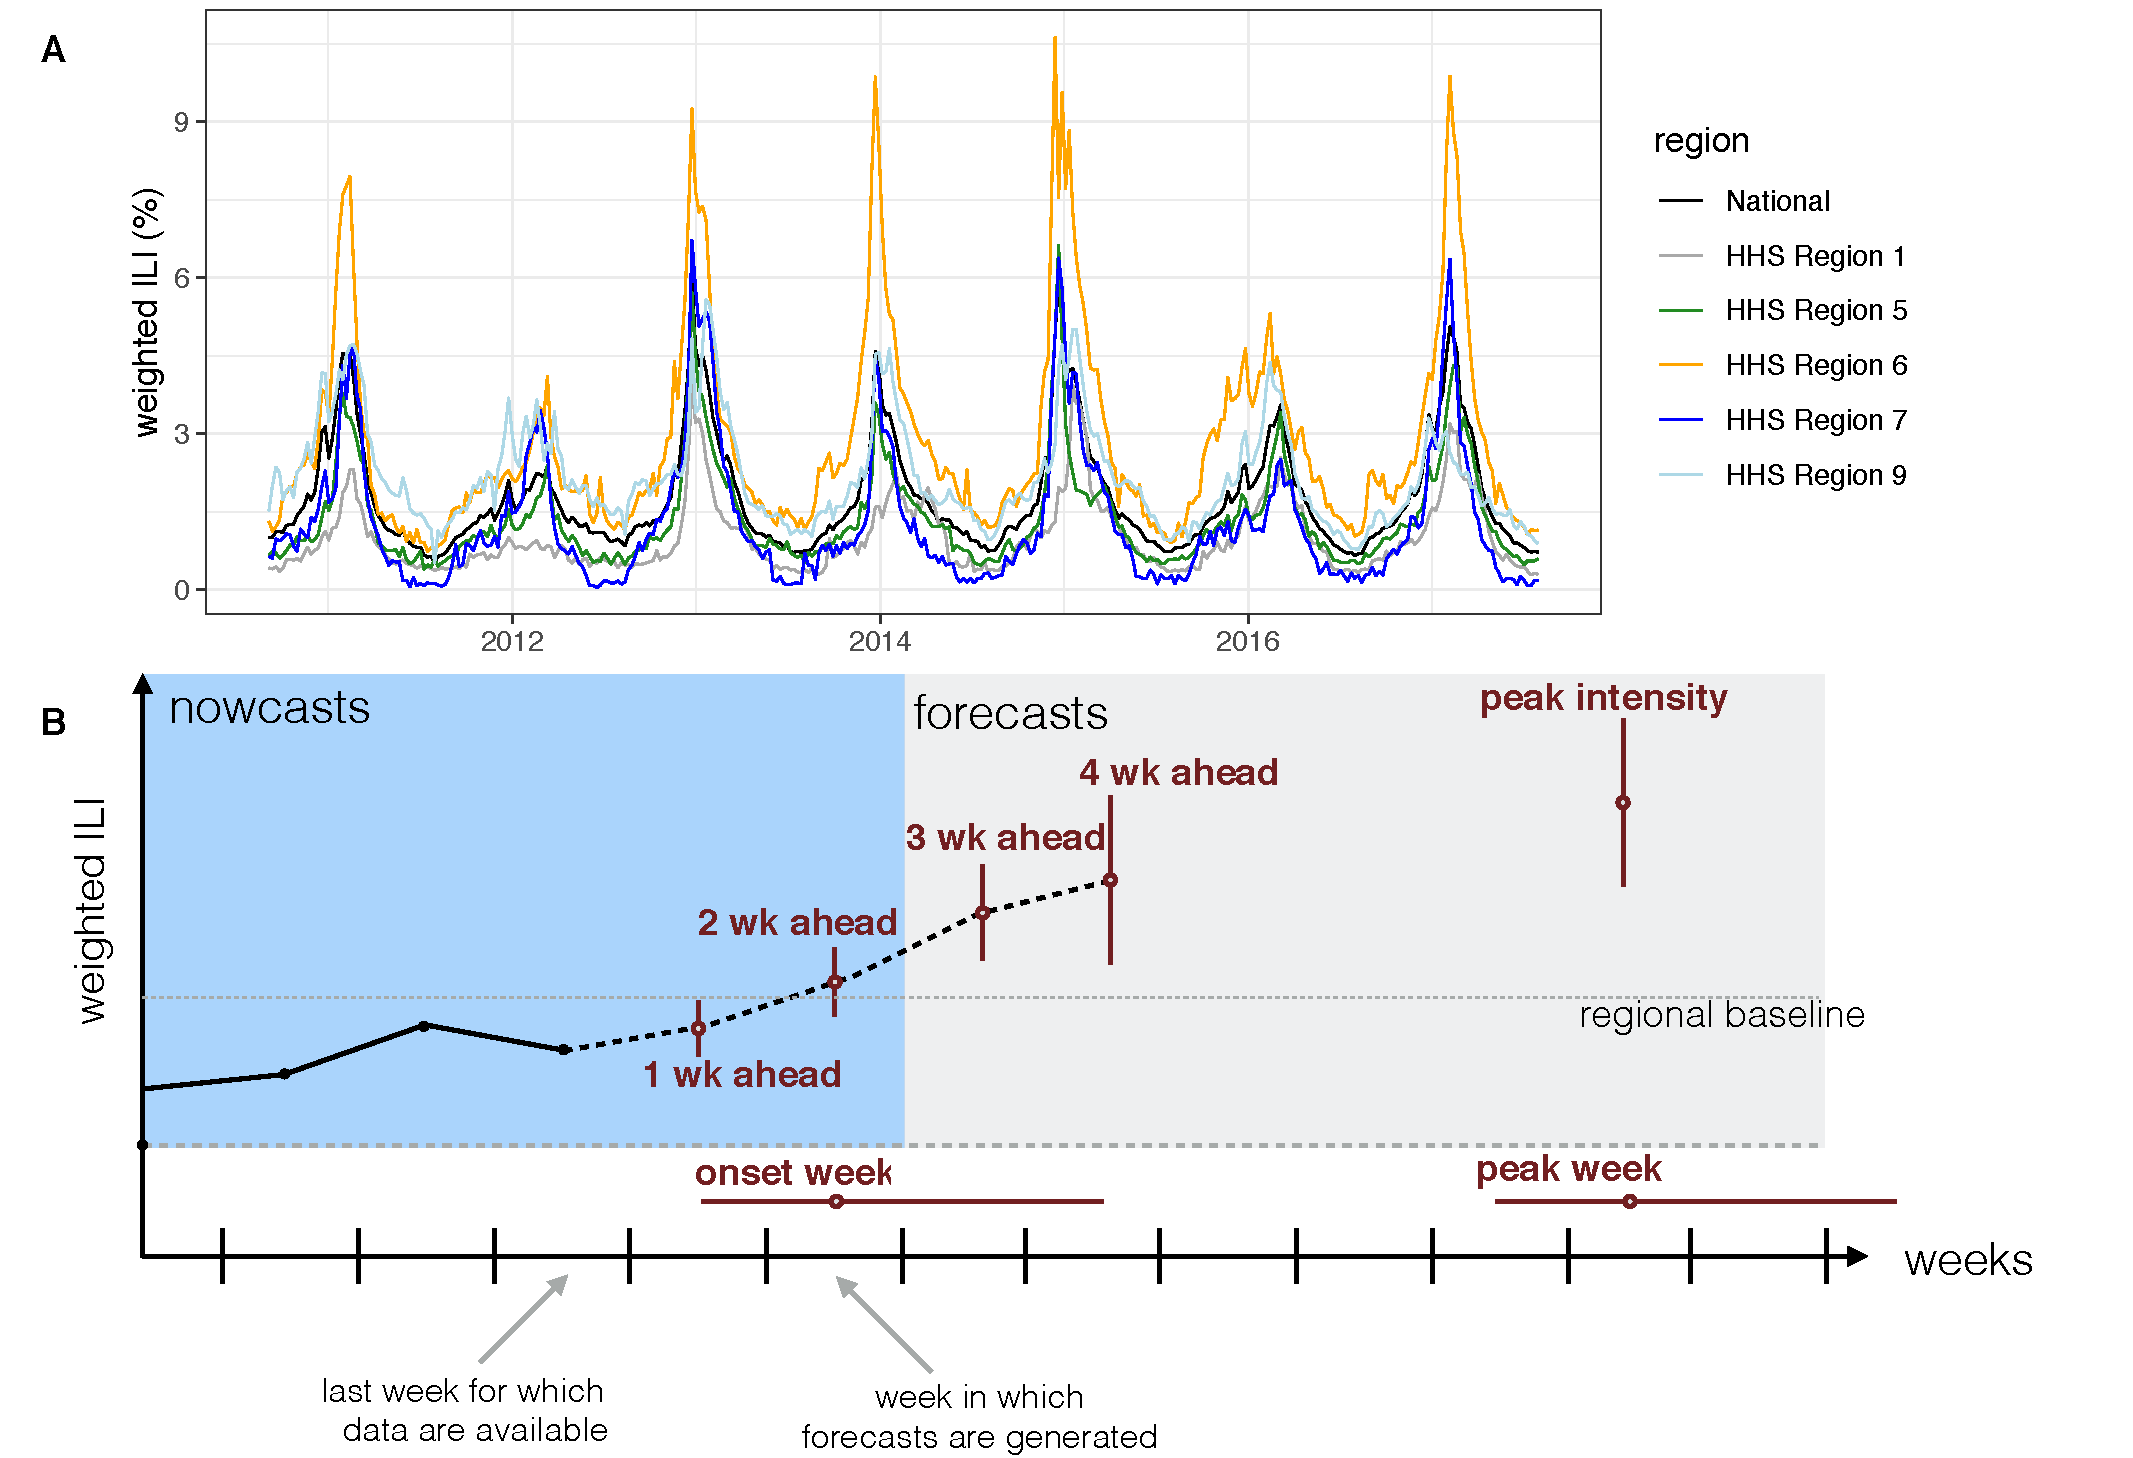
\includegraphics[width=\textwidth]{static-figures/timezero-sketch.pdf}
\caption{(A) Weighted influenza-like illness data downloaded from the CDC website. The y-axis shows the weighted percentage of doctor's office visits where the patient had influenza-like illness for each week between September 2010 through July 2017, which is the time period for which the models presented in this paper made seasonal forecasts. (B) A diagram showing the anatomy of a single forecast. The seven forecasting targets are illustrated with a point estimate (dot) and interval (uncertainty bars). The five targets on the wILI scale are shown with uncertainty bars spanning the vertical wILI axis, while the two targets for a time-of-year are illustrated with horizontal uncertainty bars along the temporal axis. The onset is defined relative to a region- and season-specific baseline wILI percentage defined by the CDC. Arrows illustrate the timeline for a typical forecast for the CDC FluSight challenge, assuming that forecasts are generated or submitted to the CDC using the most recent reported data. This data includes the first reported observations of wILI\% from two weeks prior. Therefore, 1 and 2 week-ahead forecasts are referred to as nowcasts, i.e. at or before the current time. Similarly, 3 and 4 week-ahead forecasts are forecasts, or estimates about events in the future.}
\label{fig:intro-schematic}
\end{center}
\end{figure}


\begin{Schunk}
\begin{Sinput}
> ## code for plot in Figure 1
> regionflu <- get_flu_data("hhs", sub_region=1:10, data_source="ilinet", years=1997:2017)
> usflu <- get_flu_data("national", sub_region=NA, data_source="ilinet", years=1997:2017)
> ## make AGE cols in usflu integer data type
> cols <- grepl('^AGE', colnames(regionflu))
> regionflu[,cols] <- sapply(regionflu[,cols], as.integer)
> cols <- grepl('^AGE', colnames(usflu))
> usflu[,cols] <- sapply(usflu[,cols], as.integer)
> fludata <- bind_rows(regionflu, usflu)
> fludata <- dplyr::transmute(fludata,
+     region.type = `REGION TYPE`,
+     region = REGION,
+     year = YEAR,
+     week = WEEK,
+     caldate = as.POSIXct(MMWRweek2Date(YEAR, WEEK)),
+     weighted_ili = as.numeric(`% WEIGHTED ILI`))
> fludata$region[fludata$region == "X"] <- "National"
> fludata$region <- factor(fludata$region, 
+     levels=c("National", paste("Region", 1:10)),
+     labels=c("National", paste("HHS Region", 1:10)))
> cls <- c("black", "darkgrey", "forestgreen", "orange", "blue", "lightblue")
> fludata %>%
+     filter(
+         region %in% c("National", paste("HHS Region", c(1,5,6,7,9))),
+         caldate > as.POSIXct(as.Date("2010-09-01")),
+         caldate < as.POSIXct(as.Date("2017-08-01"))) %>%
+     ggplot(aes(x=caldate, y=weighted_ili, color=region)) + 
+     xlab(NULL) + ylab("weighted ILI (%)") +
+     geom_line() +
+     #scale_color_brewer(palette="Dark2")
+     #scale_color_manual(values=brewer.pal(6, "Dark2")[c(1, 4, 3, 2, 5, 6)])
+     scale_color_manual(values=cls)
\end{Sinput}
\end{Schunk}


The FluSight challenges have defined seven forecasting targets of particular public health relevance. Three of these targets are fixed scalar values for a particular season: onset week, peak week, and peak intensity (i.e. the maximum observed wILI percentage). The remaining four targets are the observed wILI percentages in each of the subsequent four weeks (Figure \ref{fig:intro-schematic}B). 

The FluSight challenges have also required that all forecast submissions follow a particular format. A single submission file (a comma-separated text file) contains the forecast made for a particular epidemic week (EW) of a season. Standard CDC definitions of epidemic week are used. Each file contains binned predictive distributions for seven specific targets across the 10 HHS regions of the US plus the national level. Each file contains over 8000 rows and typically is about 400KB in size.

To be included in the model comparison presented here, previous participants in the CDC FluSight challenge were invited to provide out-of-sample forecasts for the 2010/2011 through 2016/2017 seasons.
For each season, files were submitted for EW40 (using standard CDC defined epidemic weeks \cite{NewMexicoDepartmentofHealth,Niemi2015,Tushar2018}) of the first calendar year of the season through EW20 of the following calendar year. 
(For seasons that contained an EW53, an additional file labeled EW53 was included.)
For each model, this involved creating 233 separate forecast submission files, one for each of the weeks in the seven training seasons.
Each forecast file represented a single submission file, as would be submitted to the CDC challenge. 
Each team created their submitted forecasts in a prospective, out-of-sample fashion, i.e. fitting or training the model only on data available before the time of the forecast (see Figure \ref{fig:intro-schematic}). 
Some data sources (e.g. wILI data prior to the 2014/2015 season) were not archived in a way that made data reliably retrievable in this ``real-time'' manner. In these situations, teams were still allowed to use these data sources with best efforts made to ensure forecasts were made using only data available at the time forecasts would have been made.

\subsection{Summary of Models}

Five teams each submitted between 1 and 9 separate models for evaluation (Table \ref{tab:model-list}). 
A wide range of methodological approaches and modeling paradigms are included in the set of forecast models.
For example, seven of the models utilize a compartmental structure (e.g. Susceptible-Infectious-Recovered), a model framework that directly encodes both the transmission and the susceptible-limiting dynamics of infectious disease outbreaks.
Other less directly mechanistic models use statistical approaches to model the outbreak phenomenon directly by incorporating recent incidence and seasonal trends.
Six models directly incorporate external data (i.e. not just the wILI measurements from the CDC ILINet dataset), including historical humidity data and Google search data.
Two models stand out as being clear baseline models, that never change based on recent data. 
The {\tt Delphi-Uniform} model always provides a forecast that assigns equal probability to all possible outcomes. 
The {\tt ReichLab-KDE} model yields predictive distributions based entirely on data from other seasons using kernel density estimation (KDE) for seasonal targets and a generalized additive model with cyclic penalized splines for weekly incidence.
Throughout the manuscript when we refer to the `historical baseline` model we mean the {\tt ReichLab-KDE} model.
Once submitted to the central repository, the models were not updated or modified except in four cases to fix explicit bugs in the code that yielded numerical problems with the forecasts. 
(In all cases, the updates did not substantially change the performance of the updated models.)
Re-fitting of models or tuning of model parameters was explicitly discouraged to avoid unintentional overfitting of models.

\begin{table}
\setlength{\tabcolsep}{4pt} 
\begin{tabular}{p{1.69cm} l p{7.5cm}  p{1.70cm}  p{1.7cm}}
\hline
Team     & Model Abbr& Model Description & External Data & Comp. Model* \\ 
\hline
CU       & EAKFC\_SEIRS       & Ensemble Adjustment Kalman Filter SEIRS                                                        & x             & x                   \\ 

~        & EAKFC\_SIRS        & Ensemble Adjustment Kalman Filter SIRS                                                         & x             & x                   \\
~        & EKF\_SEIRS         & Ensemble Kalman Filter SEIRS                                                                   & x             & x                   \\
~        & EKF\_SIRS          & Ensemble Kalman Filter SIRS                                                                    & x             & x                   \\
~        & RHF\_SEIRS         & Rank Histogram Filter SEIRS                                                                    & x             & x                   \\
~        & RHF\_SIRS          & Rank Histogram Filter SIRS                                                                     & x             & x                   \\
~        & BMA                & Bayesian Modeling Average                                                                      & ~             & ~                   \\
\hline
Delphi   & BasisRegression    & Basis Regression (epiforecast package defaults)                                                & ~             & ~                   \\ 
~        & DeltaDensity1      & Delta Density (epiforecast package defaults)                                                   & ~             & ~                   \\ 
~        & EmpiricalBayes1    & Empirical Bayes (conditioning on past four weeks only)                                         & ~             & ~                   \\ 
~        & EmpiricalBayes2    & Empirical Bayes (epiforecast package defaults)                                                 & ~             & ~                   \\ 
~        & EmpiricalFuture    & Empirical Futures (epiforecast package defaults)                                               & ~             & ~                   \\ 
~        & EmpiricalTraj      & Empirical Trajectories (epiforecast package defaults)                                          & ~             & ~                   \\ 
~        & DeltaDensity2      & Markovian Delta Density (epiforecast package defaults)                                         & ~             & ~                   \\ 
~        & Stat               & Statistical Ensemble (using the eight submitted components, with no backcasting or nowcasting) & ~             & ~                   \\
~        & Uniform            & Uniform Distribution                                                                           & ~             & ~                   \\ 
\hline
LANL     & DBM                & Dynamic Bayesian Model with a hierarchical discrepancy                                         & ~             & x                   \\ 
\hline
ReichLab & KCDE               & Kernel Conditional Density Estimation                                                          & ~             & ~                   \\ 
~        & KDE                & Kernel Density Estimation                                                                      & ~             & ~                   \\ 
~        & SARIMA1            & SARIMA model without seasonal differencing                                                     & ~             & ~                   \\ 
~        & SARIMA2            & SARIMA model with seasonal differencing                                                        & ~             & ~                   \\ 
\hline
UTAustin & EDM                & Empirical Dynamic Model                                                                        & ~             & ~                   \\ 
\end{tabular}
\caption{List of models, with key characteristics. *Comp. model stands for compartmental model.}
\label{tab:model-list}
\end{table}

\subsection{Metric Used for Evaluation and Comparison}

Influenza forecasts have been evaluated by the CDC primarily using a variation of the log-score, a measure that enables evaluation of both the precision and accuracy of a forecast.\cite{Gneiting2007} 
The log-score for a model $m$ is defined as $\log f_m(z^*|\bf{x})$ where $f_m(z|\bf{x})$ is the predicted density function from moel $m$ for some target $Z$, conditional on some data $\bf{x}$ and $z^*$ is the observed value of the target $Z$. 
The log-score is a ``proper`` scoring rule, which has the practical implication that linear combinations (i.e. arithmetic means) of log scores will also be proper.

Consistent with the primary evaluation performed by the CDC, we used a modified form of the log-score to evaluate forecasts. 
The modified log-scores are computed for the targets on the wILI percentage scale such that predictions within +/- 0.5 percentage points are considered accurate, i.e. modified log score = $\log \int_{z^* -.5}^{z^* + .5} f_m(z|{\bf{x}})dz$. 
For the targets on the scale of epidemic weeks, predictions within +/- 1 week are considered accurate, i.e. modified log score = $\log \int_{z^* -1}^{z^* + 1} f_m(z|{\bf{x}})dz$. 
While this modification means that the resulting score is not formally a proper scoring rule, some have suggested that improper scores derived from proper scoring rules may, with large enough sample size, have negligible differences in practice.\cite{Gneiting2007} % see especially last paragraph of section 2.3 
Additionally, this modified log score has the advantage of having a clear interpretation and was  motivated and designed by public health officials.
Hereafter, we will refer to these modified log scores as simply log scores.

Average log scores can be used to compare models' performance in forecasting for different locations, seasons, targets, or times of season.
In practice, each model $m$ has a set of log scores associated with it are region-, target-, season-, and week-specific.
We represent one specific scalar log score value as $\log f_{m,r,t,s,w}(z^*|\bf{x})$. 
These values can be averaged across any of the indices to create a summary measure of performance.
For example,
\begin{eqnarray}
LS_{m,\cdot,t,\cdot,\cdot} & = & \frac{1}{N} \sum_{r,s,w} \log f_{m,r,t,s,w}(z^*|{\bf x})
\end{eqnarray}
represents a log score for model $m$ and target $t$ averaged across all regions, seasons and weeks.

While log scores are not on a particularly interpretable scale, a simple transformation enhances interpretability substantially.
Exponentiating an average log score yields a forecast score equivalent to the geometric mean of the probabilities assigned to the eventually observed outcome. 
The geometric mean is an alternative measure of central tendency to an arithmetic mean, representing the $N^{th}$ root of a product of $N$ numbers. 
Using the example above, we then have that
\begin{eqnarray}
S_{m,\cdot,t,\cdot,\cdot} = \exp \left ( LS_{m,\cdot,t,\cdot,\cdot} \right ) & = & \exp \left ( \frac{1}{N} \sum_{r,s,w} \log f_{m,r,t,s,w}(z^*|{\bf x}) \right ) \\
 & = & \left ( \prod_{r,s,w}  f_{m,r,t,s,w}(z^*|{\bf x}) \right ) ^{1/N} 
\end{eqnarray}
In this setting, this score has the intuitive interpretation of being the average probability assigned to the true outcome (where average is considered to be a geometric average).
Hereafter, we will refer to an average score as an exponentiated average log score.
In all cases, we compute the averages arithmetically on the log scale and only exponentiate before reporting and interpreting a final number
Therefore, all reported average scores can be interpreted as the corresponding geometric means, or as the correponding average probabilities assigned to the true outcome.

Following the convention of the CDC challenges, we only included certain weeks in the calculation of the average log scores for each target.
This focuses model evaluation on periods of time that are more relevant for public health decision making.
Forecasts of season onset are evaluated based on the forecasts that are received up to six weeks after the observed onset week within a given region.
Peak week and peak intensity forecasts were scored for all weeks in a specific region-season up until the wILI measure drops below the regional baseline level for the final time. 
(All weeks are scored if wILI never goes above the baseline.)
%Forecasts of season peak and intensity are evaluated through the first forecast received after the weighted ILI goes below the regional baseline for the final time during a given region-season. 
Week-ahead forecasts are evaluated using forecasts received four weeks prior to the onset week through forecasts received three weeks after the weighted ILI goes below the regional baseline for the final time.
In a region-season without an onset, all weeks are scored.
To ensure all calculated summary measures would be finite, all modified log scores with values of less than -10 were assigned the value -10, following CDC scoring conventions.
All scores were based on ``ground truth'' values of wILI data obtained as of September 27, 2017.

% \subsection{Formal comparisons of model performance}
% 
% Model-based comparisons of forecast accuracy are hindered by the high correlation of sequential forecasts and by outlying observations. 
% When observations assign no probability to the eventually observed outcome they have a log-score of $-\infty$.

%Things to confirm: removed weeks that CDC does not score, no onset seasons and multi peak years are handled appropriately

\subsection{Specific model comparisons}\label{sec:delay-model}

\subsubsection*{Analysis of data revisions}
% from fig-delay-model-coefs.R
% fm4 <- glm(exp(multi_bin_score) ~ Model + Target + factor(forecasted_epiweek) + bias_first_report_factor, data=scores_for_analysis)

The CDC publicly releases data on doctor's office visits due to ILI each week. 
These data for previous weeks (especially the most recent ones) are occasionally revised, due to new or updated data being reported to the CDC since their last report.
While often these revisions are fairly minor or non-existent, at other times, these revisions can be substantial, changing the reported wILI value by over 50\% of the originally reported value.
Since these data are used by forecasters to generate current forecasts, these forecasts can be contaminated by the initially reported, biased data.

We used a regression model to analyze the impact of these unrevised reports on forecasting.
Specifically, for each region and epidemic week we calculated the difference between the first and the last reported ILI values for each epidemic week for which forecasts were generated in the seven seasons under consideration.
We then created a categorical variable ($X$) with a binned representation of these differences using the following six categories covering the entire range of obesrved values: (-3.5,-2.5], (-2.5,-1.5], ..., (1.5,2.5].
Using the forecasting results from the four most accurate individual non-ensemble models, ({\tt ReichLab-KCDE}, {\tt LANL-DBM}, {\tt Delphi-DeltaDensity1}, {\tt CU-EKF\_SIRS}), we then fit the following linear regression model
\begin{equation}
S_i = \beta + \alpha_{m(i)} + \gamma_{t(i)} + \lambda_{w(i)} + {\mathbf \theta}\cdot X_i + \epsilon_i
\end{equation}
where the index $i$ indexes a specific set of subscripts $\{m,r,t,s,w\}$, and the $\alpha_{m(i)}$, $\gamma_{t(i)}$, and $\lambda_{w(i)}$ are model-, target-, and week-specific fixed effects, respectively. (The notation $m(i)$ refers to the model contained in the ith observation of the dataset.) The error term is assumed to follow a Gaussian distribution with mean zero and an estimated variance parameter. The parameter of interest in the model is the vector ${\mathbf \theta}$, which represent the expected changes in average score from the reference category (defined as the bin representing changes of between +/- 0.5 from the original reported value) adjusting for model, target and week-of-season.

\subsubsection*{Mechanistic vs. statistical models}

% Infectious disease modeling has proven to be fertile ground for statisticians, mathematicians, and quantitative modelers for over a century. 
There is not a consensus on a single best modeling approach or method for forecasting the dynamic patterns of infectious disease outbreaks, in both endemic and emergent settings. 
Semantically, modelers and forecasters often use a dichotomy of mechanistic vs. statistical (or `phenomenological') models to represent two different philosophical approaches to modeling.
Mechanistic models for infectious disease consider the biological underpinnings of disease transmission, and are in practice are implemented as variations on the Susceptible-Infectious-Recovered (SIR) model. 
Statistical models largely ignore the biological underpinnings and theory of disease transmission and focus instead on using data-driven, empirical and statistical approahces to make the best forecasts possible of a given dataset, or phenomenon. 

However, in practice, this dichotomized distinction is less clear than it is in theory.
For example, statistical models for infectious disease counts may encode an autoregressive term for incidence (i.e. as done by the {\tt ReichLab-KCDE} model).
This could be interpreted as representing a transmission process from one time period to another.
In another example, the {\tt LANL-DBM} model has an explicit SIR compartmental model component but also leverages a hierarchical discrepancy which is purely statistical.
The models from Columbia University used a statistical `now-casting' approach for their 1-week ahead forecasts, but after that relied on different variations of an SIR model.
% Both approaches are commonly used and both have advantages and disadvantages in different settings.  

We categorized models according to whether or not they had any explicit compartmental framework (Table \ref{tab:model-list}). 
We then took the top three performing compartmental models (i.e. models with some kind of an underlying compartmental structure) and compared their performance with the top three individual component models without compartmental structure. 
We excluded multi-model ensemble models (i.e. {\tt Delphi-Stat}) from this comparison.
Separately for each target, we computed the average score for the top three compartmental models and compared this to the average score for the top three non-compartmental models.

\subsection{Reproducibility and data availability}

To maximize the reproducibility and data availability for this project, the data and code for the entire project (excluding specific model code) are publicly available.
The project is available on GitHub\cite{fsngithub2018}, with a permanent repository [[stored on Zotero]].
All of the forecasts may be interactively browsed on the website http://flusightnetwork.io.
A web applet with interactive visualizations of the model evaluations is available at https://ermoore.shinyapps.io/FSN\_Model\_Comparison/. [[link to change]]
Additionally, this manuscript was dynamically generated using R version 3.4.2 (2017-09-28), Sweave, and knitr, tools for intermingling manuscript text with R code that run the central analyses, minimizing the chances for errors transcribing or translating results.\cite{Xie2015,RCore2017}.

\section{Results}

\subsection{Comparing models' forecasting performance by season}
\begin{Schunk}
\begin{Sinput}
> kde_logscore <- unlist(scores_by_model[which(scores_by_model$Model=="ReichLab-KDE"), "avg_logscore"])
> max_logscore <- max(scores_by_model$avg_logscore)
> min_logscore <- min(scores_by_model$avg_logscore)
> max_logscore_model <- as.character(unlist(scores_by_model[which(scores_by_model$avg_logscore == max_logscore), "Model"]))
> min_logscore_model <- as.character(unlist(scores_by_model[which(scores_by_model$avg_logscore == min_logscore), "Model"]))
> n_above_kde <- sum(scores_by_model$avg_logscore>kde_logscore)
> n_models <- nrow(scores_by_model)
> n_seasons <- nrow(scores_by_season)
> n_regions <- nrow(scores_by_region)
> tmp <- scores_by_model_season %>% group_by(Model) %>%
+     summarize(n_seasons_above_maxavg = sum(avg_logscore>max_logscore)) 
\end{Sinput}
\end{Schunk}


Averaging across targets and locations, forecast score varied widely by model and season (Figure \ref{fig:results-model-season}). 
The historical baseline model ({\tt ReichLab-KDE}) showed an average seasonal score of 
0.20, 
meaning that in a typical season, across all targets and locations, this model assigned on average 
0.20 
probability to the eventually observed value. 
The model with the highest average seasonal forecast score 
({\tt Delphi-Stat}) 
and lowest 
({\tt Delphi-EmpiricalBayes2}) 
had scores of 0.37 and 0.07, respectively. 
Of the 22 models, 16 models 
(73\%) 
showed higher average seasonal forecast score than the historical average.
Season-to-season variation was substantial, with 
10 
models having at least one season with greater average forecast score than the 
{\tt Delphi-Stat}
model did.

